% Created 2026-11-19 to 14:50
% Intended LaTeX compiler: pdflatex
\documentclass[11pt]{article}

\usepackage[utf8]{inputenc}
\usepackage[T1]{fontenc}
\usepackage{graphicx}
\usepackage{longtable}
\usepackage{wrapfig}
\usepackage{rotating}
\usepackage[normalem]{ulem}
\usepackage{amsmath}
\usepackage{amssymb}
\usepackage{capt-of}
\usepackage{hyperref}
\usepackage{listings}
\usepackage{color}
\usepackage{amsmath}
\usepackage{array}
\usepackage[T1]{fontenc}
\usepackage{natbib}
\date{\today}
\title{}
\begin{document}

\setcounter{tocdepth}{2}
\tableofcontents

The reference scenario considers two treatment protocols,
LIRA and PLACEBO, with death as the outcome.

\begin{figure}[htbp]
\centering

\includegraphics[width=.9\linewidth]{figures/rmse00.png}
\caption{Distribution of of rTMLE estimates from reference for increasing sample sizes. Dashed line indicates that of the naive estimates}
\end{figure}

\begin{figure}[htbp]
\centering
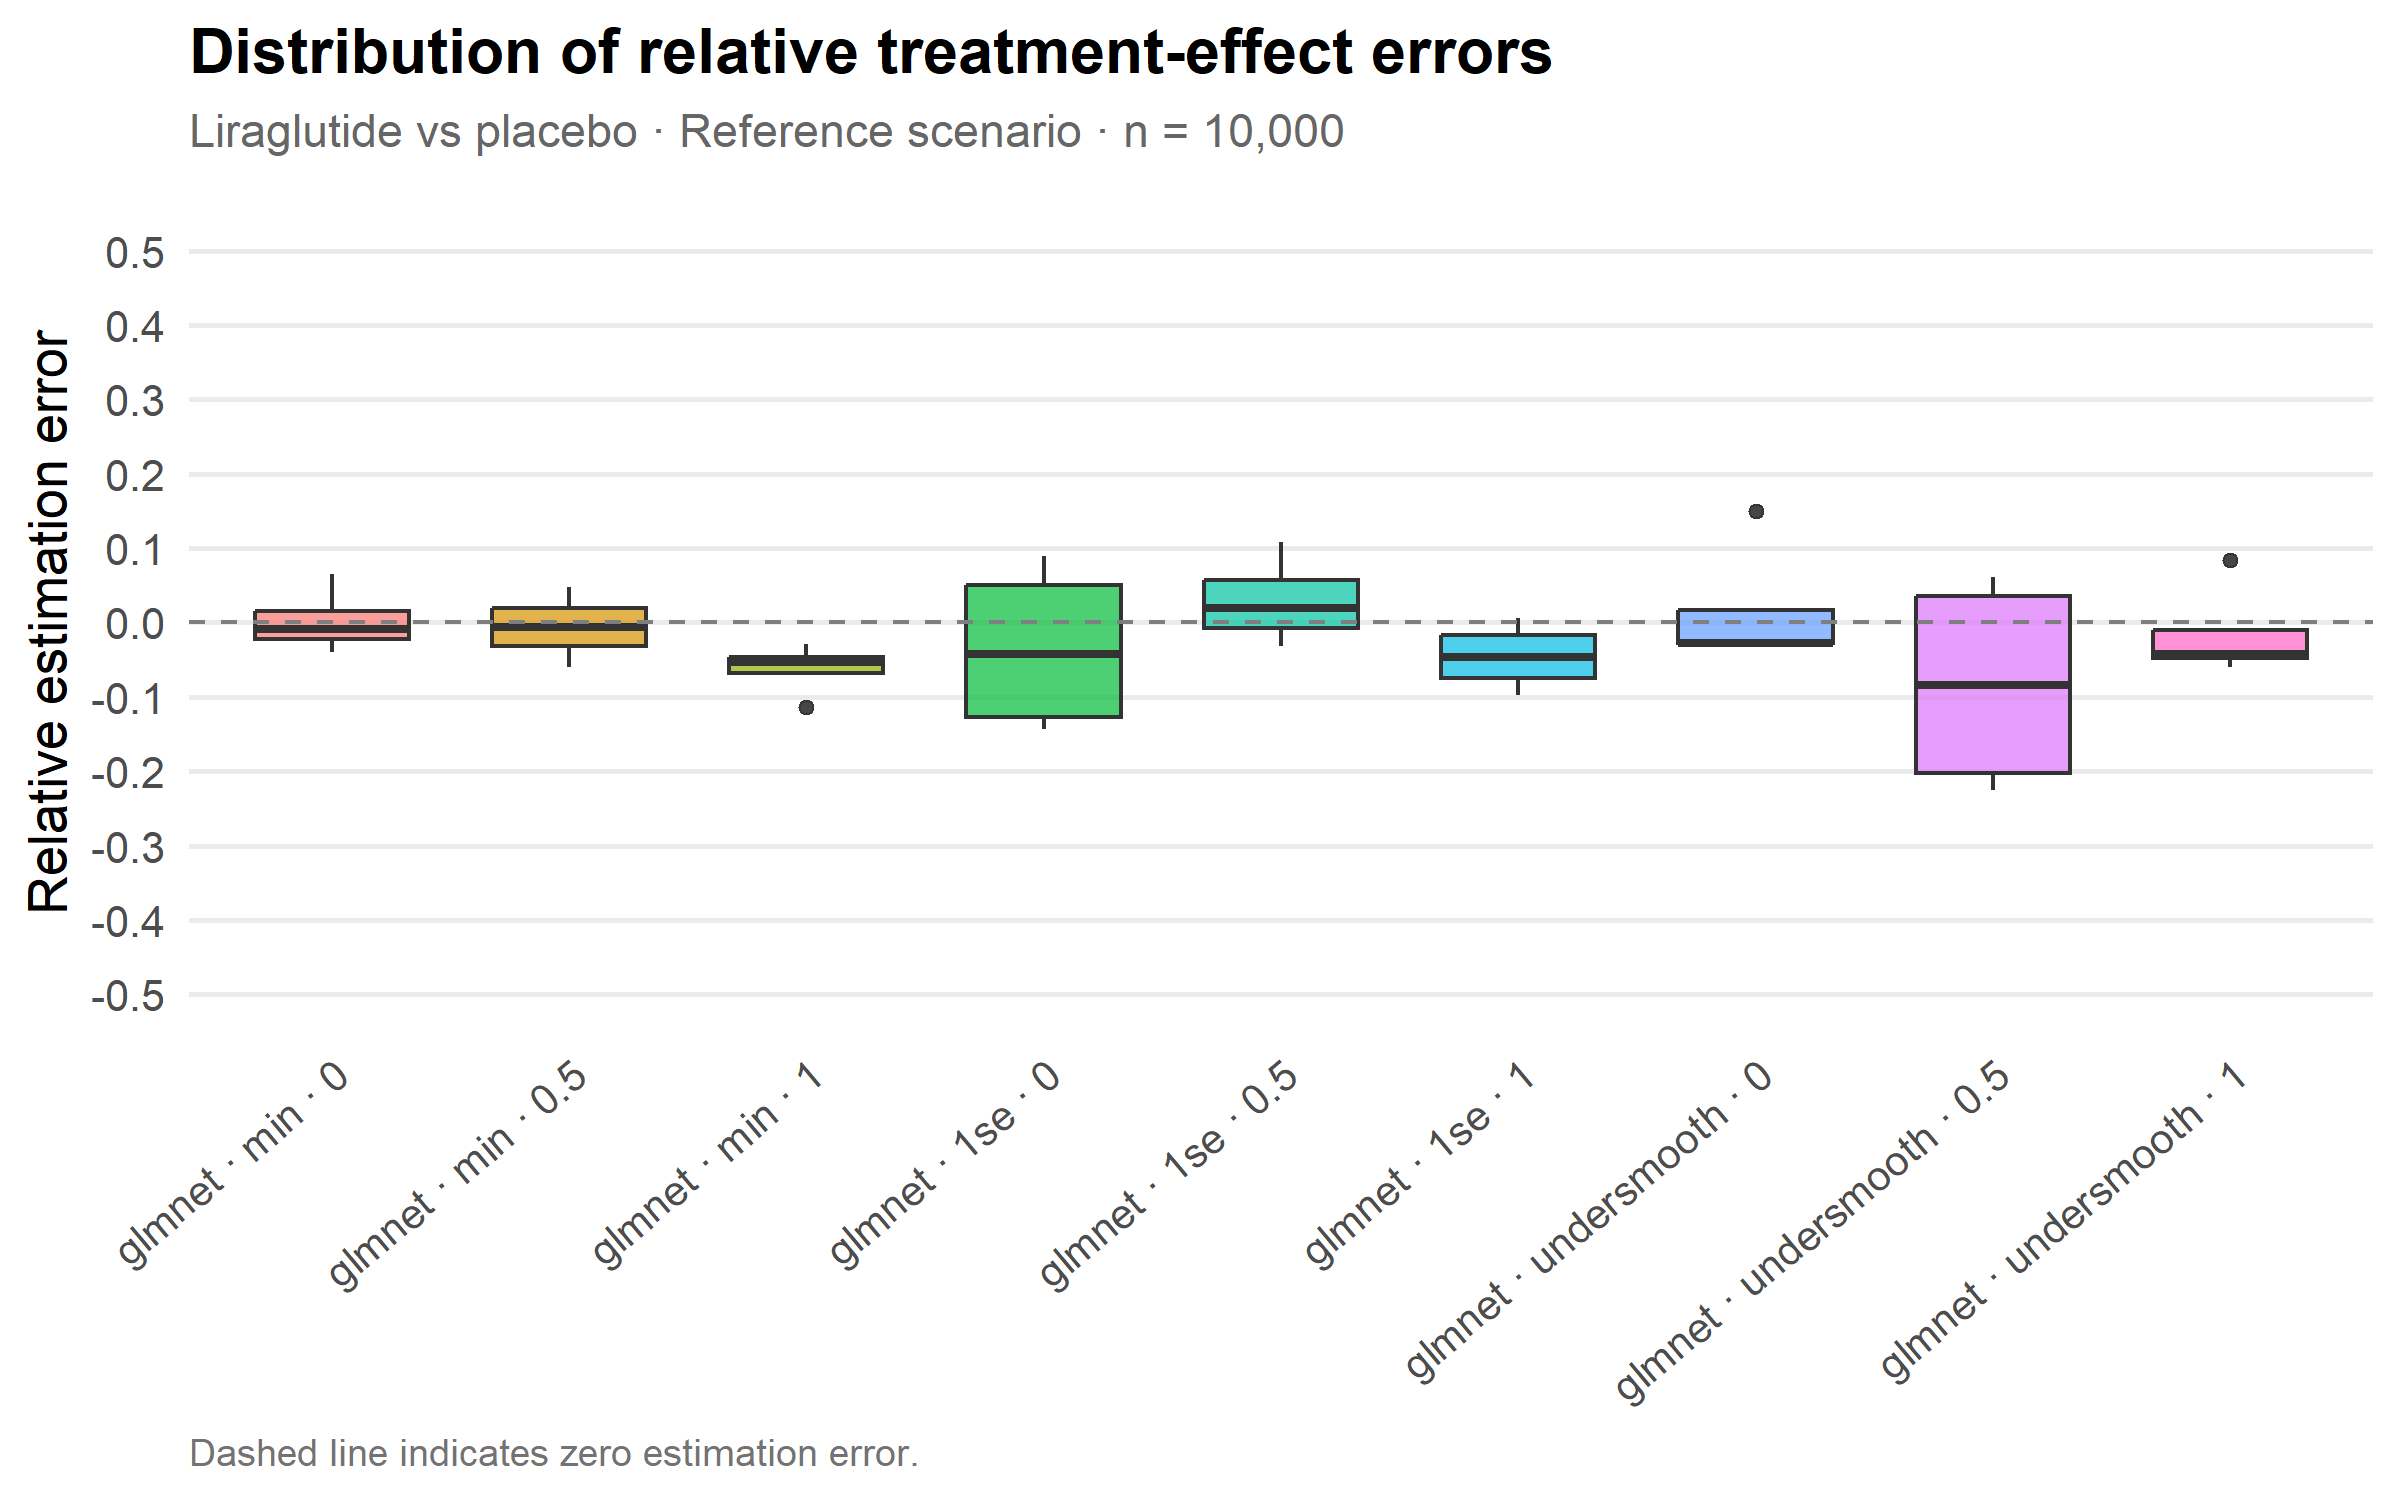
\includegraphics[width=.9\linewidth]{figures/boxplot00.png}
\caption{Distribution of between estimate and reference across simulations}
\end{figure}





Then, an additional absorbing outcome (censoring) is introduced in the form of
dropout. The 

\begin{figure}[htbp]
\centering
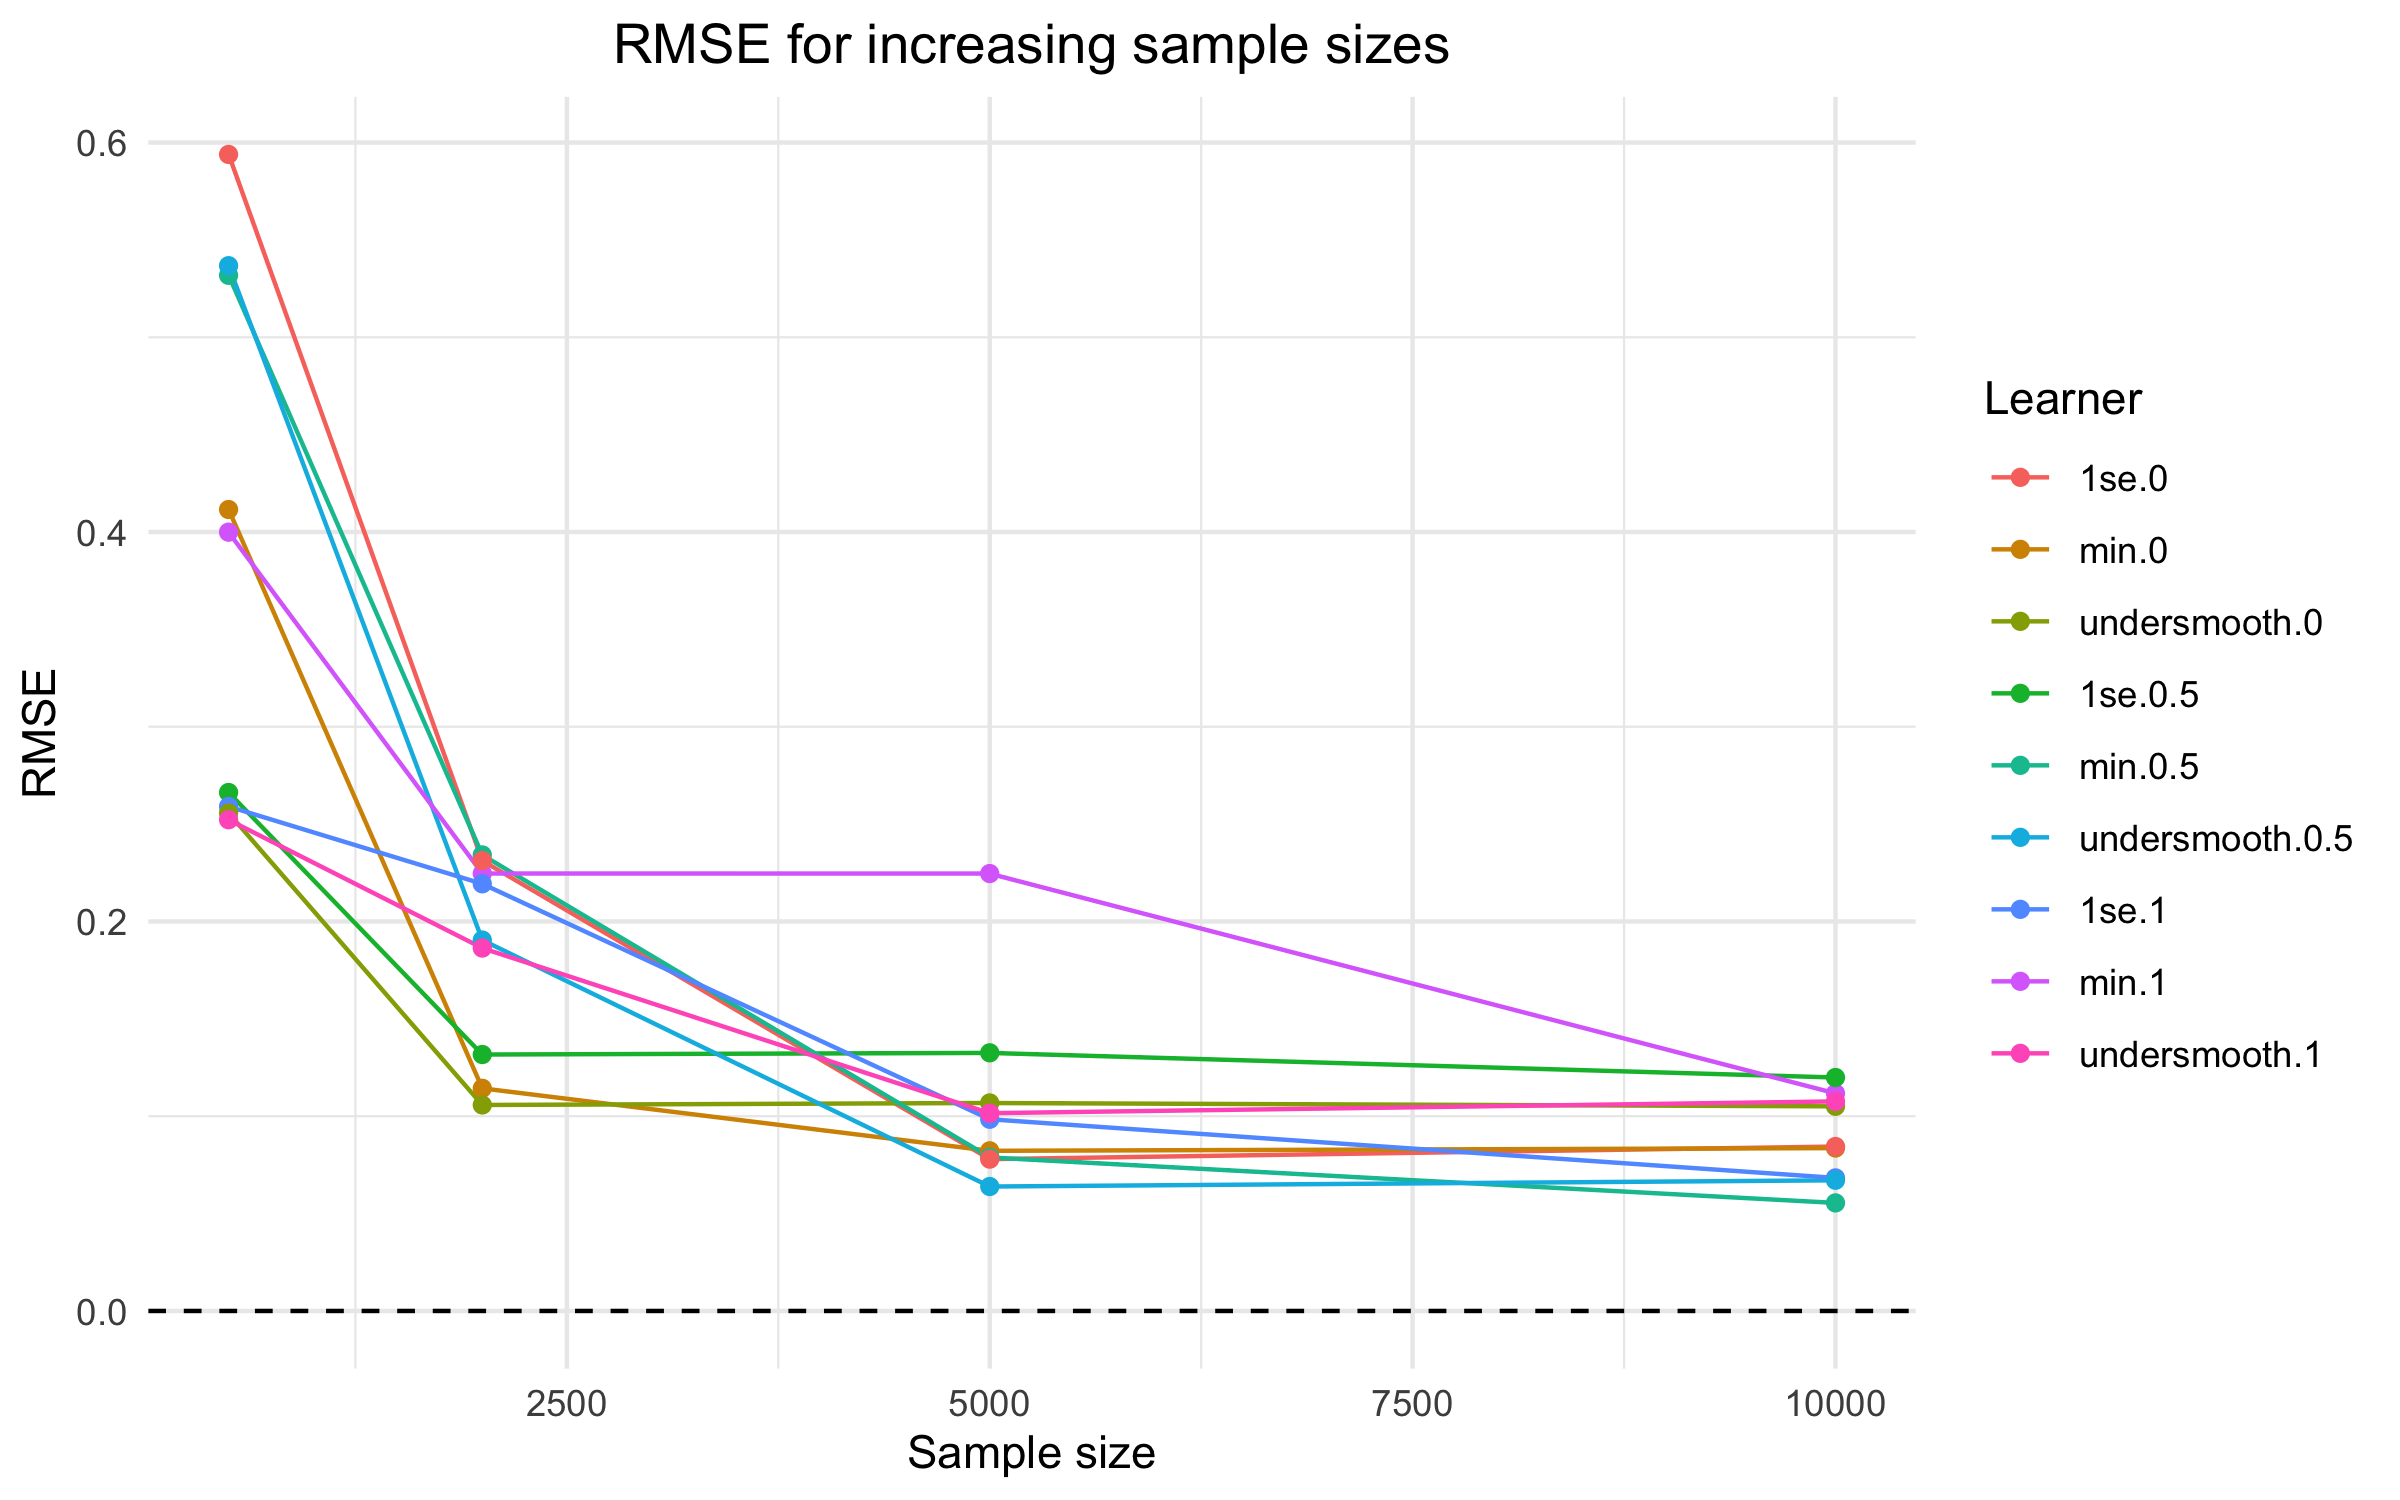
\includegraphics[width=.9\linewidth]{figures/rmse0ce.png}
\caption{Distribution of of rTMLE estimates from reference for increasing sample sizes. Dashed line indicates that of the KM estimates}
\end{figure}

\begin{figure}[htbp]
\centering
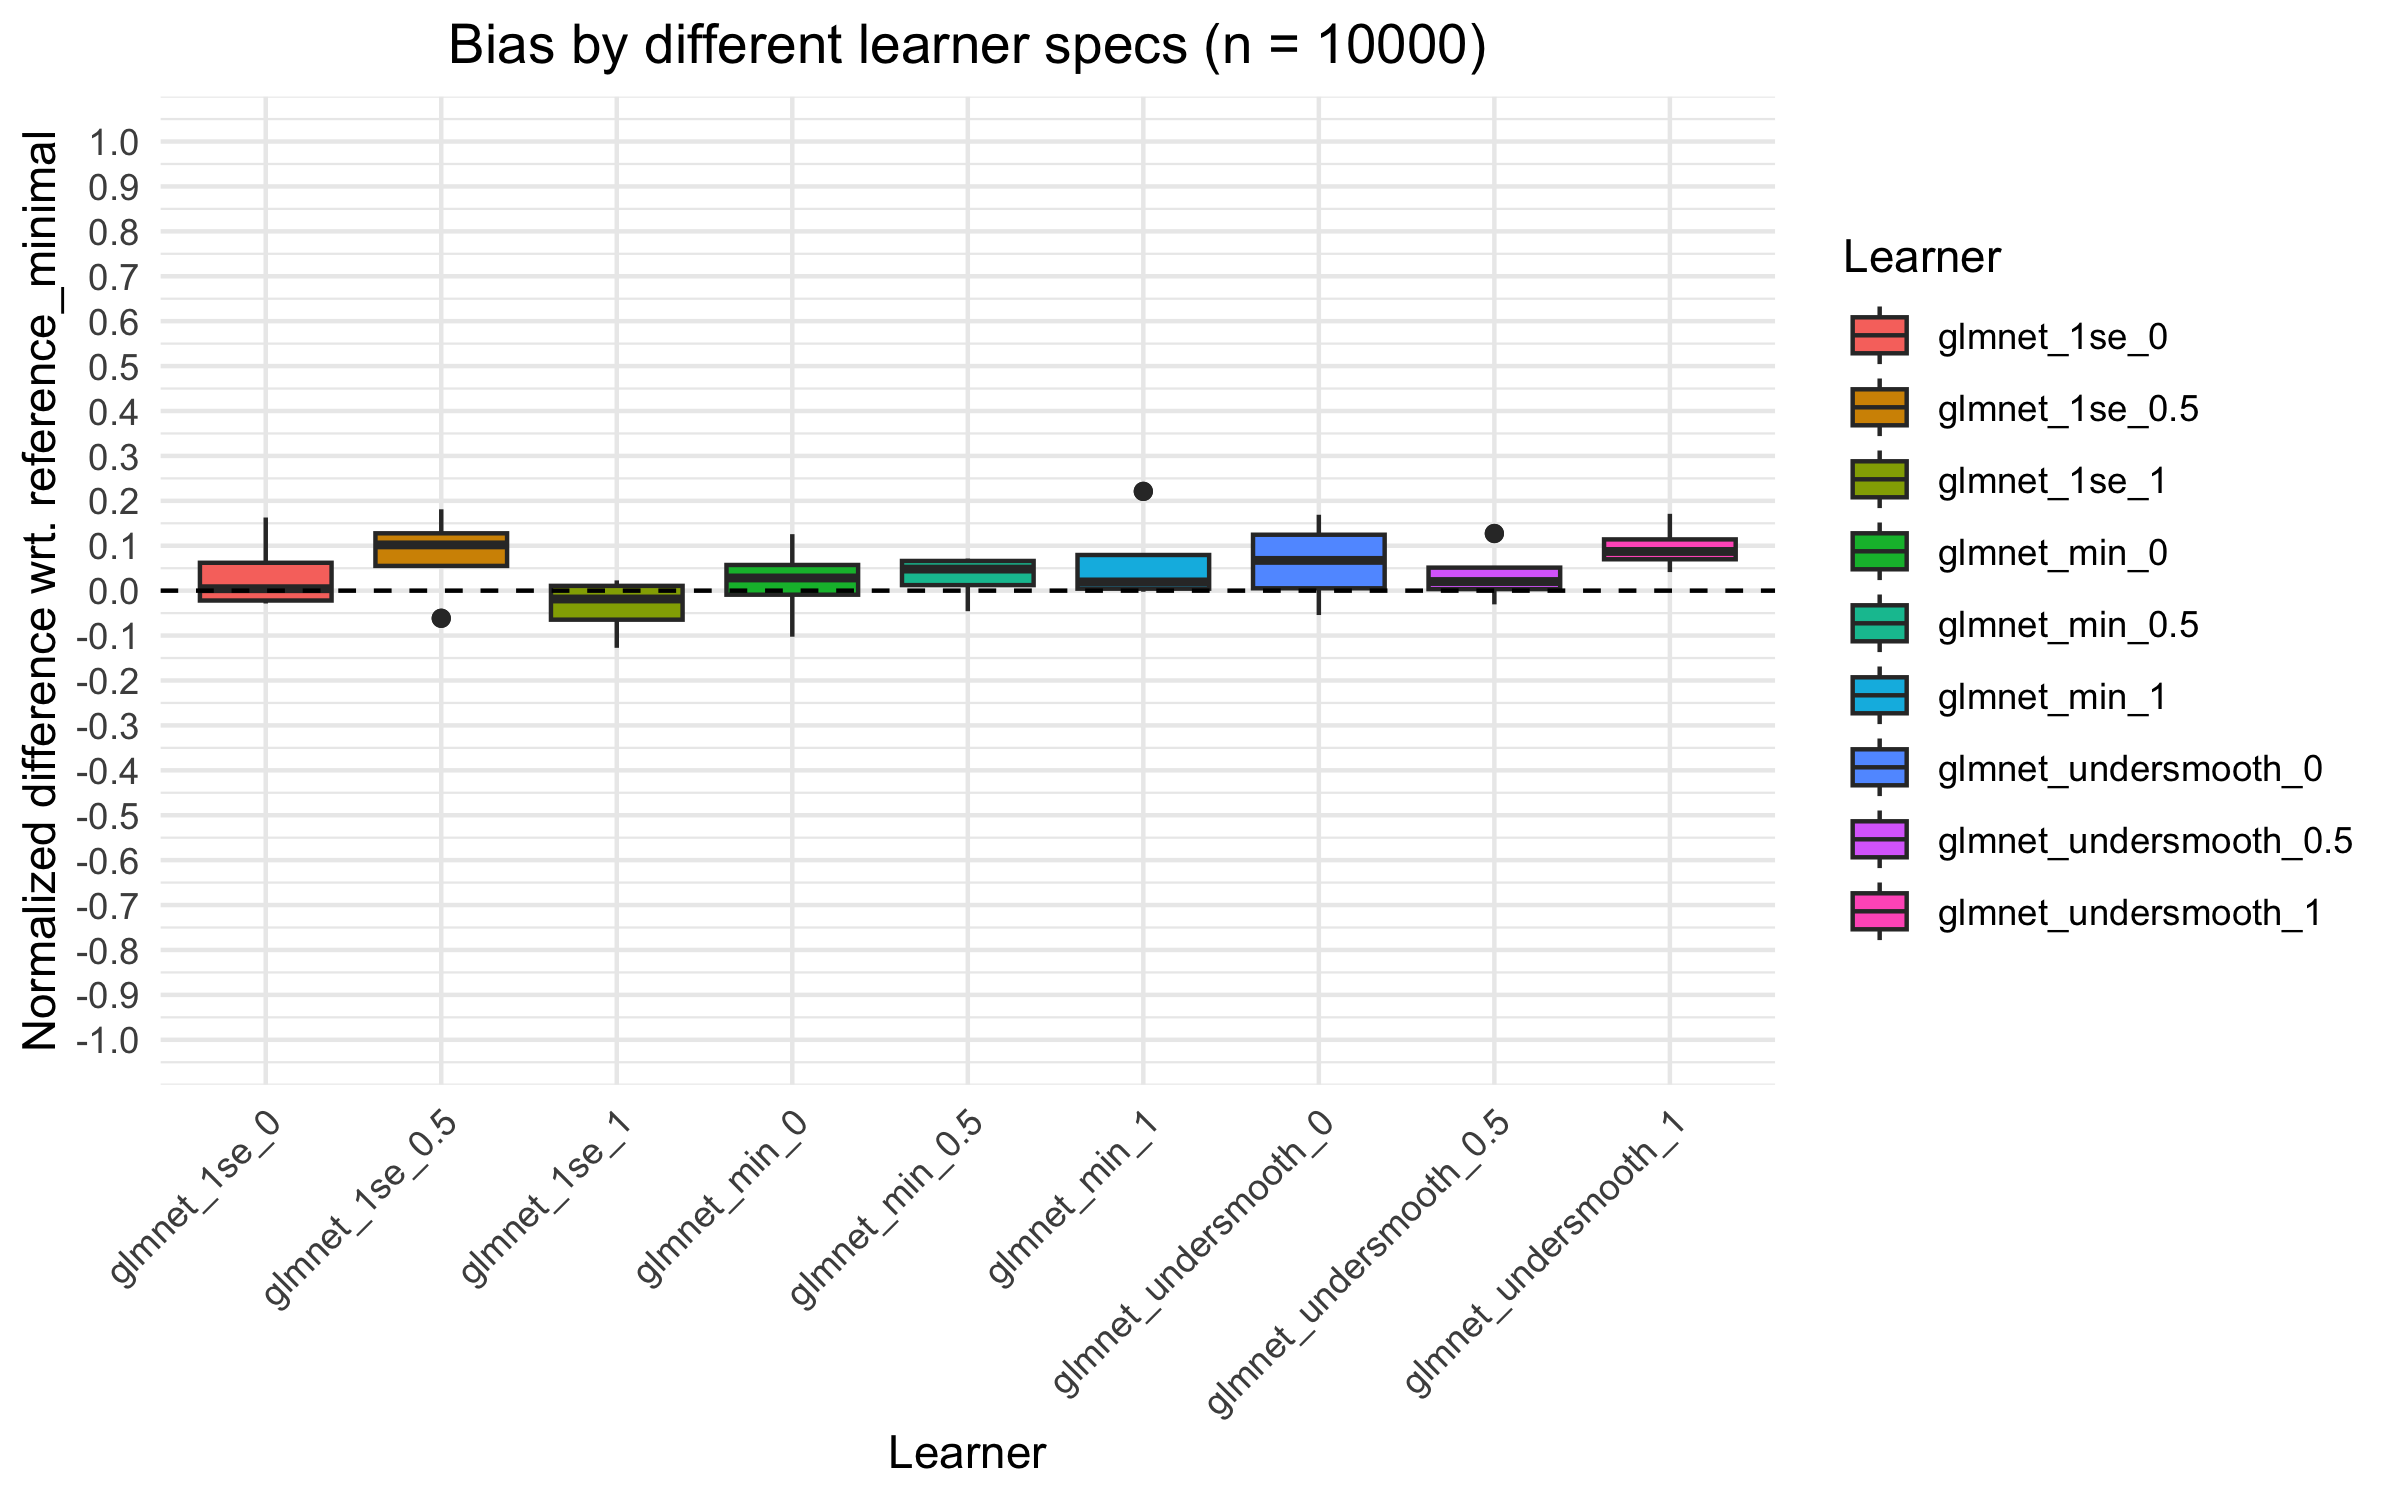
\includegraphics[width=.9\linewidth]{figures/boxplot0ce.png}
\caption{Distribution of estimate and reference across simulations}
\end{figure}

Then, confounding.

Then, both censoring and confounding.
\end{document}
